\documentclass{article}
\usepackage{graphicx} % Required for inserting images
\usepackage{hyperref} % Required for crosslink
\usepackage{subcaption} % Required for subcaption for figures
\usepackage{multirow} % Required for multirow in table
\usepackage{amsmath}
\usepackage{listings}
\usepackage{minted}
\usepackage{caption} % Required for left table name 
\usepackage{biblatex}
\usepackage{indentfirst}
\usepackage{pgfplots} % plot
\usepackage{xcolor}
\usepackage{tikz}
\usepackage{fourier} 
\usepackage{array}
\usepackage{makecell}
\usepackage[colorlinks]{hyperref}

\addbibresource{ref.bib} 

\title{The Parallelization of Explicit In-time and Two Dimensional Finite Difference Solver Using MPI}
\author{Mehmet Şamil Dinçer (2236248)\\
        Elvin Gültekinoğlu (2446169)}
\date{January 2024}

\begin{document}

\maketitle

\section{Abstract}

The Message Passing Interface is an acknowledged standard for distributed computing and it is commonly utilized in different solvers used in several problems. The idea behind MPI is based on dividing the problem into nodes, synchronizing the action of parallel nodes and providing data exchange between different cores. In that sense, the term Message Passing points out the use of MPI in data transfer. One application of MPI is the parallelization of the explicit in-time, two-dimensional finite difference solver which tackles the wave equation. In this paper, this implementation is explained in detail pointing out important characteristics of MPI. 
\clearpage

\section{Introduction}

Parallel programming has gained an important place in engineering applications to solve equations relating physical phenomena in a shorter time and a systematic way. In that sense, different standards have been set for solving such equations by parallelizing the processes. The Message Passing Interface (MPI) is an application program interface which has an extensive use these days. In Bruck et al. (1995) \cite{bruck1995efficient}, MPI is defined as an industrial standard based on writing portable message-passing parallel programs. In MPI, each parallel unit has its own local memory and data is shared between these units. In one paper, Skjellum et al. (1994) \cite{skjellum1994extending} explains MPI as encompassing point-to-point and collective message passing, communication scoping and virtual topologies within the scope of a model of distributed computing. At that point, it should be pointed out that MPI provides flexibility and practicality in parallel programming. \\

The explicit in-time, two dimensional, finite difference solver used to solve the wave equation employs point-to-point communication relating processors through MPI. This solver requires a special attention in implementing MPI since this is a two dimensional solver. After parallelizing the serial code given previously, the parallel code is compiled and run by specifying the number of cores. Here the main idea is to provide a condition according to the specified core number such that each processor has the same number of nodes. As an output, the infinity norm of the error and the time taken along with the number of processors are printed out. \\

The performance evaluation of the code is considered by running the code with different configurations. These are mesh resolutions and number of processors. In addition to these, strong scaing analysis is performed by fixing the problem size. \\

Throughout this paper, the implementation of MPI on a solver which tackles the wave equation is explained in detail along with important aspects. The comments are also made on the corresponding performance parameters to observe the effect of parallelization and the use of MPI inclusively. All these are provided and summarized at the end of the paper. 

\clearpage 

\section{The Theory and Methodology} 
This section extensively elaborates on the solver's theoretical foundation, the approach used to incorporate MPI in deatil. 
\subsection{The Solver}
The focus of this paper is explicit in-time, two-dimensional, finite difference solver which handles the wave equation. This equation is given in Equation \ref{the_main_solver}. In this equation, c is a non-negative real real constant, q is the field variable and t is the time. 
\begin{equation}  
    \frac{{\partial q}^2}{{\partial t}^2} = c^2 \left(\frac{{\partial q}^2}{{\partial x}^2} + \frac{{\partial q}^2}{{\partial y}^2}\right)
    \label{the_main_solver}
\end{equation}
The wave equation is a second order linear partial differential equation which is used to describe the behavior of mechanical and electromagnetic waves. Examples of such waves are sound waves, water waves and light waves. \\

This solver is two-dimensional as mentioned earlier, so there are two space variables to define the overall region which are x and y. The limiting values for x and y are read from the input file through the prepared code. The number of nodes in x and y directions are also obtained from the same input file. The number of nodes in these two directions are the same and they are referred to as global node numbers (NX \& NY). Solution parameters such as the start time, the end time and the time step size are also read and kept so as to be used in further steps. \\

The domain decomposition is performed to provide the same number of nodes per processor. This decomposition is performed in one chosen direction only since the solver consists of two dimensions. In this case, y direction is chosen as the one on which the decomposition is performed. It is important to note that x direction stands for the horizontal axis while y direction refers to the vertical axis adhering to the right hand rule. In that sense, local node number variables are defined for two directions as given in Equations \ref{local_node_numbers_x} and \ref{local_node_numbers_y}. 
\begin{equation}  
    nx = NX 
    \label{local_node_numbers_x}
\end{equation}
\begin{equation}  
    ny = NY/size
    \label{local_node_numbers_y}
\end{equation}
Here lower cases refer to local variables and upper cases refer to global ones obtained from the input file. Since the decomposition is only performed for one of the axes, local node number in x direction is equal to the global node number in the same direction. However, this is not the case for y direction. In that axis, global node number is divided by the total number of cores such that in each processor, the same number of nodes is present. The decomposition for four cores is observed in Figure \ref{figure_1}. As seen in this figure, the domain is divided into sub-parts by using the aforementioned equations.\\

\begin{figure}[hbt!]
    \centering
    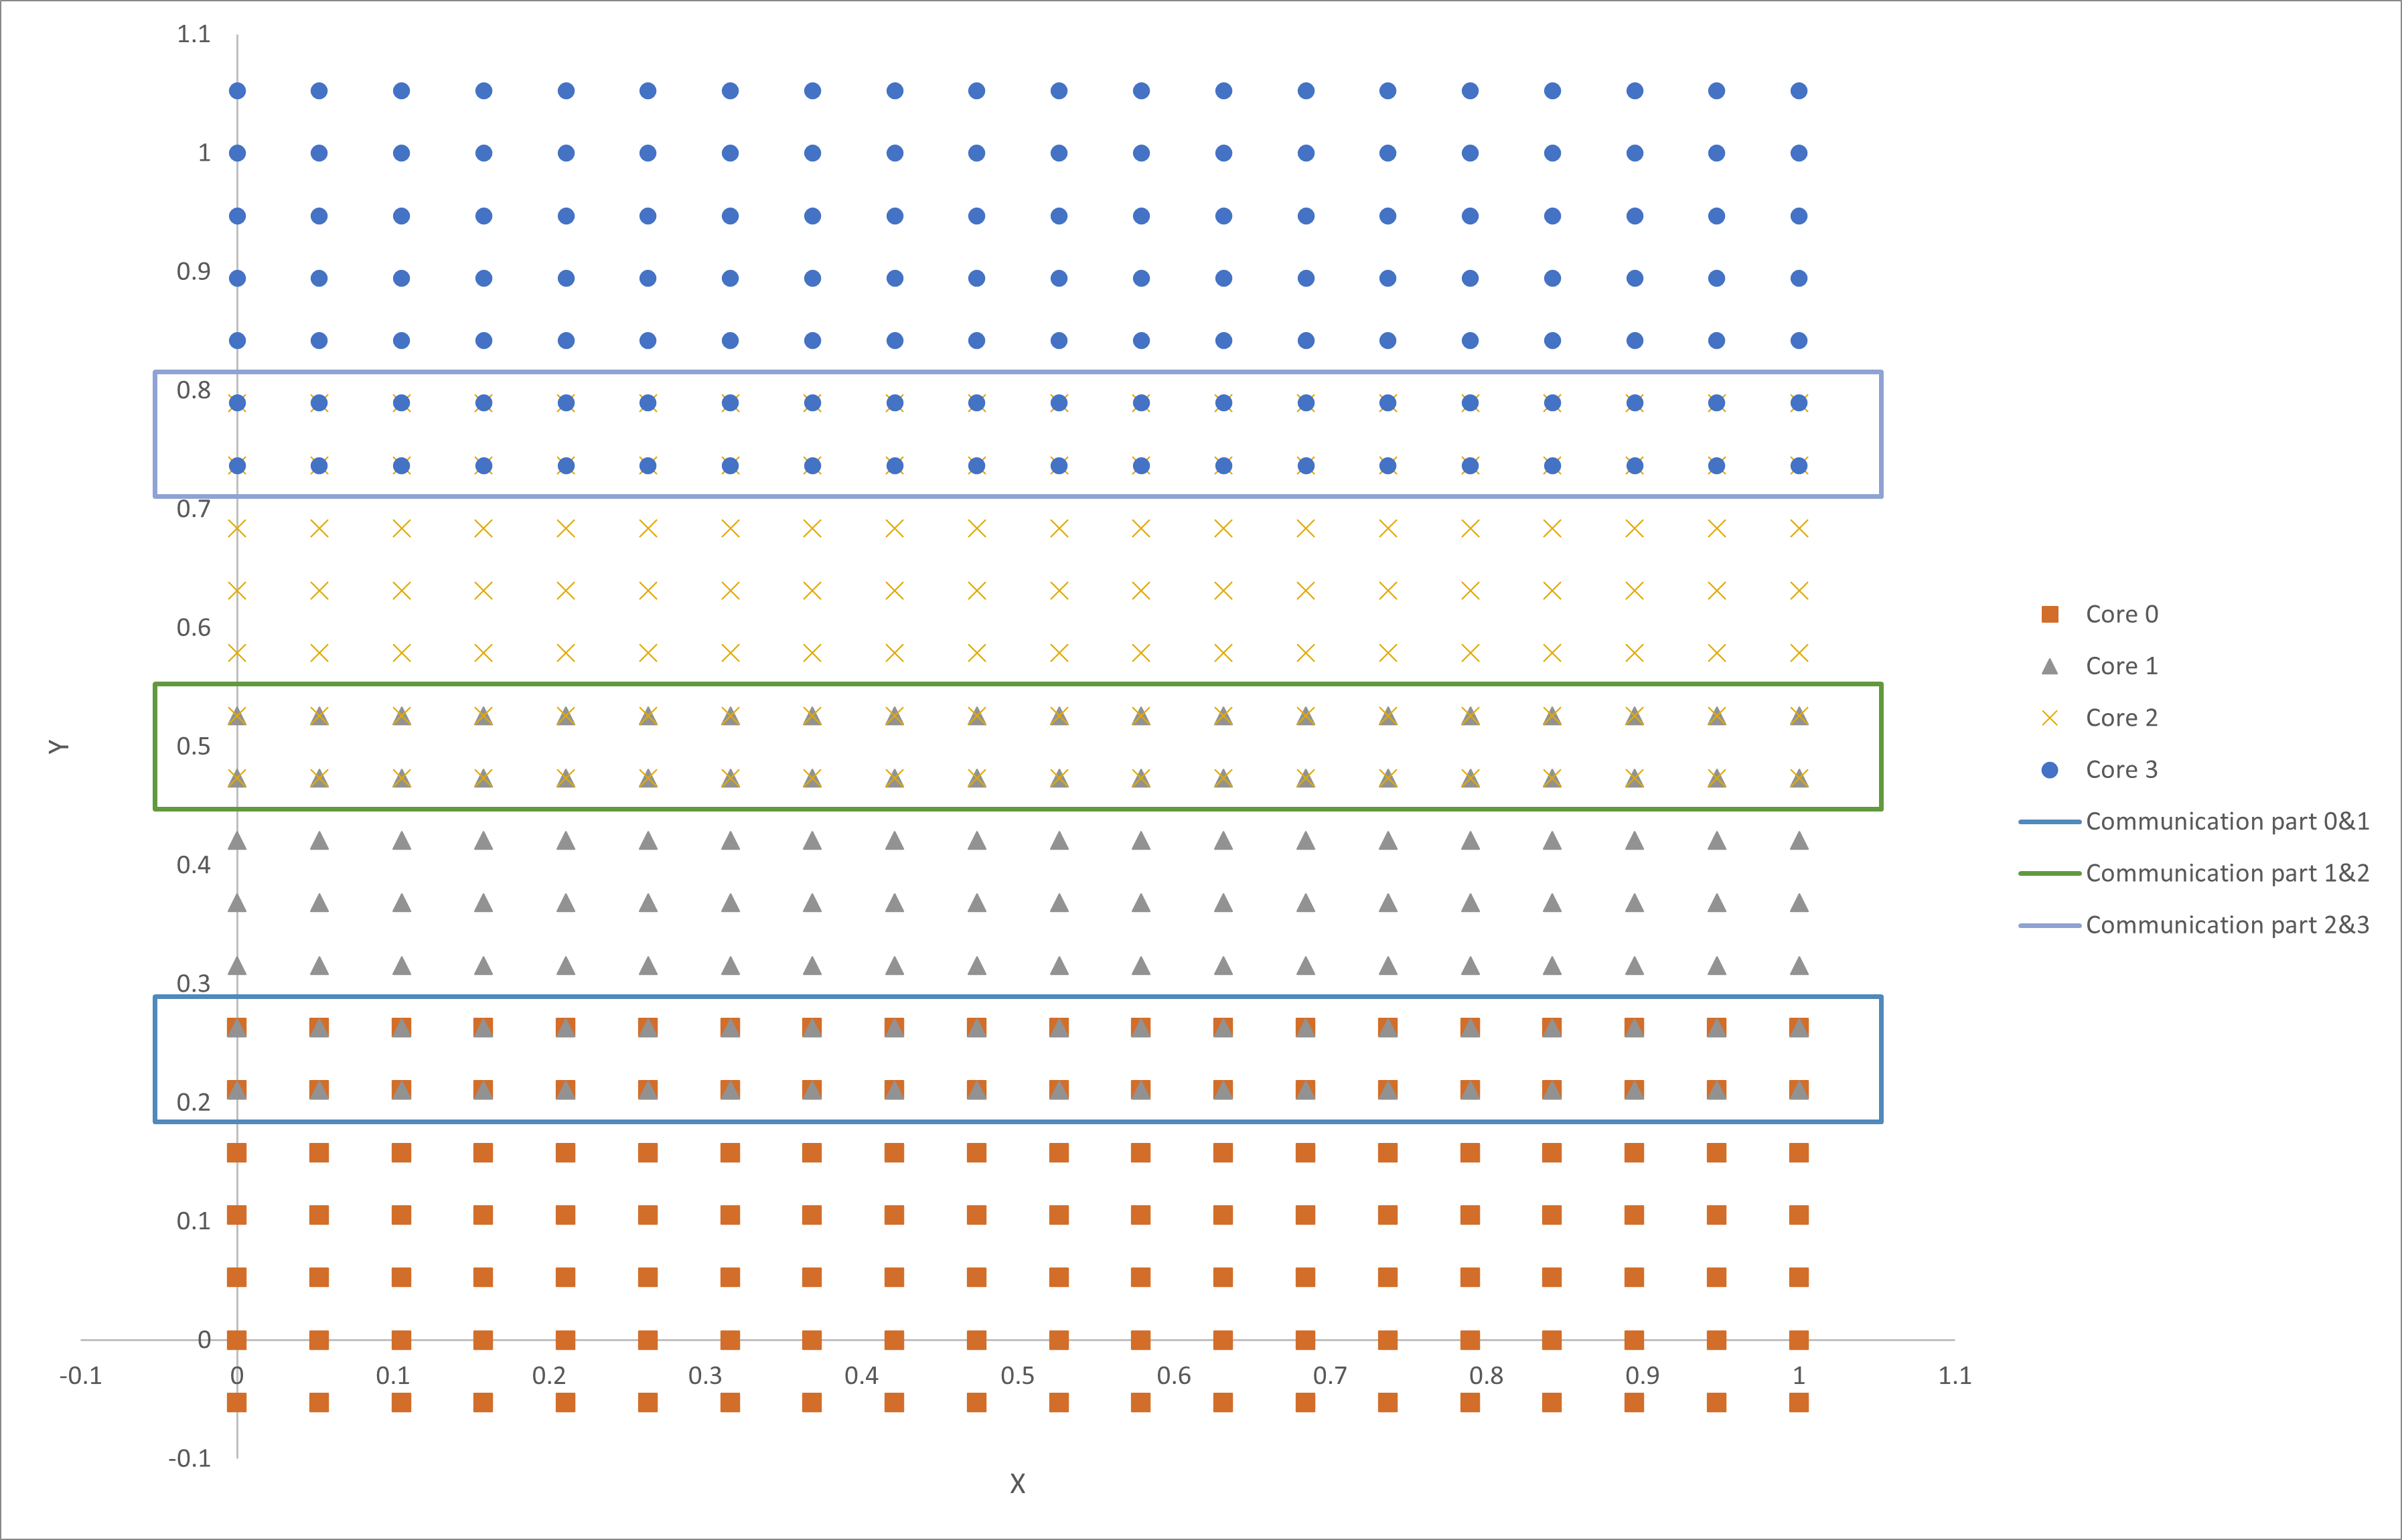
\includegraphics[width=1\textwidth]{Figures/decomposion.png}
    \caption{The Domain Decomposition}
    \label{figure_1}
\end{figure}
The uniform spacing in x and y directions are calculated as given in Equations \ref{uniform_spacing_x} and \ref{uniform_spacing_y}. In these equations, x\textunderscore max and x\textunderscore min represent preset limits in x direction. The same representation holds for y direction also. Under these restrictions, the spacing for the domain is obtained which is used to compute the coordinates of each point in the same domain. 
\begin{equation} % Diffisuion equation 
    hx = \frac{x\textunderscore max - x\textunderscore min}{NX - 1}
    \label{uniform_spacing_x}
\end{equation}
\begin{equation} % Diffisuion equation 
     hy = \frac{y\textunderscore max - y\textunderscore min}{NY - 1}
    \label{uniform_spacing_y}
\end{equation}
The coordinates of each node are calculated in a sequential manner by using previously calculated uniform spacing in x and y directions and also the index of current process. The formulations are provided in Equations \ref{local_node_numbers_x} and \ref{local_node_numbers_y}. 
\begin{equation} % Diffisuion equation 
    x[i+j*nx] = i*hx 
    \label{x_points}
\end{equation}
\begin{equation} % Diffisuion equation 
     y[i+j*nx]= -hy + ( j*hy) + (rank * hy * ny)
    \label{y_points}
\end{equation}
Letters i and j refer to the current local node numbers starting from zero to "nx" and "ny+2". Here "ny+2" is taken instead of "ny" directly which is the case in the serial solver. This is due to the point-to-point communication which comes with MPI implementation. The implementation of this part in the code is given below. 
\definecolor{mygray}{rgb}{0.95,0.95,0.95}
\begin{minted}[autogobble=true, frame=lines, framesep=4mm, baselinestretch=1.2, bgcolor=mygray, fontsize=\footnotesize, linenos=true, breaklines]{c}
// Compute coordinates of the nodes
  for(int j=0; j < ny+2; ++j){
    for(int i=0; i < nx;++i){
      x[i+j*nx]= ( i*hx); 
      y[i+j*nx]= -hy + ( j*hy) + (rank * hy * ny) ;
    }
  }
\end{minted}
\subsection{The Implementation of MPI}
It is expected to implement MPI on a given code by using point-to-point communication between processors. This part is valid when the size is bigger than one, which amounts to the number of current processes. This is such because when the size is one, end points overlap each other. For point-to-point communication, certain steps are followed. It should be noted that here q represents the field variable and it is the same variable as in Equation \ref{the_main_solver}. Since the solver is two-dimensional, three different field variables are considered. These are "qn", "q0" and "q1" which represent solution at time (t+dt), solution at time (t) and solution at time (t-dt), respectively. Before proceeding the communication section, exact solutions are recorded into q0 and q1 as the history of the field. The calculation of t is given in Equation \ref{equation_t}. Start\textunderscore time stands for the time read from input file and dt refers to time step. 
\begin{equation} % Diffisuion equation 
    t = start\textunderscore time + dt
    \label{equation_t}
\end{equation}
The implementation of communication part consists of four main steps. The idea is to manipulate communication according to the current process index referred to as rank. As seen in Item \ref{item_1}, the index of q0 is specified as the multiplication of nx and ny. As will be seen in the following lines of this paper, the number of data to be sent is set to nx. This situation is the same for the following items also. This implementation is a shortcut to send nx number of elements in one operation. \\
\begin{enumerate}
\color{black}
\item When the current process index is not equal to the very last process: q0[nx*ny] and q1[nx*ny] are sent to the next rank.
\label{item_1}
\item When the current process index is not equal to the very first process: q0[0] and q1[0] are received from the previous rank.  
\label{item_2}
\item When the current process index is not equal to the very first process again: q0[nx] and q1[nx] are sent to the previous rank. 
\label{item_3}
\item When the current process index is equal to the last process: q0[nx*(ny+1)] and q1[nx*(ny+1)] are received from the next rank. 
\label{item_4}
\end{enumerate}
The implementation of these four items in point-to-point communication inside the code is represented below. \\

\definecolor{mygray}{rgb}{0.95,0.95,0.95}
\begin{minted}[autogobble=true, frame=lines, framesep=4mm, baselinestretch=1.2, bgcolor=mygray, fontsize=\footnotesize, linenos=true, breaklines]{c}
//Communication Part 
if(size>1){

if (rank != size - 1) {
  MPI_Request send_upper_request[2];
    MPI_Isend(&q0[nx*ny], nx, MPI_DOUBLE, rank + 1, rank, MPI_COMM_WORLD, &send_upper_request[0]);
    MPI_Isend(&q1[nx*ny], nx, MPI_DOUBLE, rank + 1, rank+nx, MPI_COMM_WORLD, &send_upper_request[1]);
}
if (rank != 0) {
    //double rec;
    MPI_Request recv_lower_request[2];
    MPI_Irecv(&q0[0], nx, MPI_DOUBLE, rank - 1, rank-1, MPI_COMM_WORLD, &recv_lower_request[0]);
    MPI_Irecv(&q1[0], nx, MPI_DOUBLE, rank - 1, rank-1 + nx, MPI_COMM_WORLD, &recv_lower_request[1]);
    MPI_Waitall(2, recv_lower_request, MPI_STATUSES_IGNORE);
}
if (rank != 0) {
  MPI_Request send_lower_request[2];
    MPI_Isend(&q0[nx], nx, MPI_DOUBLE, rank - 1, rank+nx+nx-1, MPI_COMM_WORLD, &send_lower_request[0]);
    MPI_Isend(&q1[nx], nx, MPI_DOUBLE, rank - 1, rank+nx+nx+nx-1, MPI_COMM_WORLD, &send_lower_request[1]);
}
if (rank != size - 1) {
    MPI_Request recv_upper_request[2];
    MPI_Irecv(&q0[nx*(ny+1)], nx, MPI_DOUBLE, rank + 1, rank+nx+nx, MPI_COMM_WORLD, &recv_upper_request[0]);
    MPI_Irecv(&q1[nx*(ny+1)], nx, MPI_DOUBLE, rank + 1, rank+nx+nx+nx, MPI_COMM_WORLD, &recv_upper_request[1]);
    MPI_Waitall(2, recv_upper_request, MPI_STATUSES_IGNORE);
}

}
\end{minted}
Whether the size is bigger than one is checked to initiate the parallel process by communication. As seen, the number of elements to be sent and received is set as the local number of nodes, nx. The number of elements is specified such since the solver is used as two-dimensional. After performing these for all ranks, communication section is done. \\
\subsection{The Implementation of a Second Order Finite Differencing Method}
The solution is obtained by employing a second order finite differencing method at time t. In the discretization of time and space derivatives, this method is utilized as given in Equations \ref{fem_eq_t}, \ref{fem_eq_x} and \ref{fem_eq_y}. 
\begin{equation}  
    \frac{{\partial q}^2}{{\partial t}^2} = \frac{q(x,y,t + \Delta t) - 2q(x,y,t) + q(x,y,t - \Delta t)}{\Delta t^2}
    \label{fem_eq_t}
\end{equation}
\begin{equation}  
    \frac{{\partial q}^2}{{\partial x}^2} = \frac{q(x + \Delta x,y,t) - 2q(x,y,t) + q(x - \Delta x,y,t)}{\Delta x^2}
    \label{fem_eq_x}
\end{equation}
\begin{equation}  
    \frac{{\partial q}^2}{{\partial y}^2} = \frac{q(x,y + \Delta y,t) - 2q(x,y,t) + q(x,y  - \Delta y,t)}{\Delta y^2}
    \label{fem_eq_y}
\end{equation}
To utilize this method in the code, uniform spacing in time and space is implemented with a defined notation. These notations are provided on Equations \ref{eq_1}, \ref{eq_2} and \ref{eq_3}. 
\begin{equation}  
    q_{i,j}^n = q(x,y,t)
    \label{eq_1}
\end{equation}
\begin{equation}  
    q_{i+1,j}^{n+1} = q(x + \Delta x,y,t + \Delta t)
    \label{eq_2}
\end{equation}
\begin{equation}  
    q_{i,j-1}^{n-1} = q(x,y - \Delta y,t - \Delta t)
    \label{eq_3}
\end{equation}
The implementation of these notations on the mentioned method in the code is given below. 
\definecolor{mygray}{rgb}{0.95,0.95,0.95}
\begin{minted}[autogobble=true, frame=lines, framesep=4mm, baselinestretch=1.2, bgcolor=mygray, fontsize=\footnotesize, linenos=true, breaklines]{c}
// Update solution using second order central differencing in time and space
    
if(rank==0){
    for(int i=1; i<nx-1; i++){ // exclude left right boundaries
      for(int j= 2; j<ny+1 ; j++){ // exclude top and bottom boundaries
        const int n0   = i + j*nx; 
        const int nim1 = i - 1 + j*nx; // node i-1,j
        const int nip1 = i + 1 + j*nx; // node i+1,j
        const int njm1 = i + (j-1)*nx; // node i, j-1
        const int njp1 = i + (j+1)*nx; // node i, j+1
        // update solution 
        qn[n0] = 2.0*q0[n0] - q1[n0] + alphax2*(q0[nip1]- 2.0*q0[n0] + q0[nim1])
                                     + alphay2*(q0[njp1] -2.0*q0[n0] + q0[njm1]); 
      }
    }
}else if(rank==(size-1)) {
    for(int i=1; i<nx-1; i++){ // exclude left right boundaries
      for(int j= 1; j<ny ; j++){ // exclude top and bottom boundaries
        const int n0   = i + j*nx; 
        const int nim1 = i - 1 + j*nx; // node i-1,j
        const int nip1 = i + 1 + j*nx; // node i+1,j
        const int njm1 = i + (j-1)*nx; // node i, j-1
        const int njp1 = i + (j+1)*nx; // node i, j+1
        // update solution 
        qn[n0] = 2.0*q0[n0] - q1[n0] + alphax2*(q0[nip1]- 2.0*q0[n0] + q0[nim1])
                                     + alphay2*(q0[njp1] -2.0*q0[n0] + q0[njm1]); 
      }
    }
    }else {
    for(int i=1; i<nx-1; i++){ // exclude left right boundaries
      for(int j= 1; j<ny+1 ; j++){ // exclude top and bottom boundaries
        const int n0   = i + j*nx; 
        const int nim1 = i - 1 + j*nx; // node i-1,j
        const int nip1 = i + 1 + j*nx; // node i+1,j
        const int njm1 = i + (j-1)*nx; // node i, j-1
        const int njp1 = i + (j+1)*nx; // node i, j+1
        // update solution 
        qn[n0] = 2.0*q0[n0] - q1[n0] + alphax2*(q0[nip1]- 2.0*q0[n0] + q0[nim1])
                                     + alphay2*(q0[njp1] -2.0*q0[n0] + q0[njm1]); 
      }
    }
}
\end{minted}
Then the history for q1 and q0 is updated in the code as represented below. 
\definecolor{mygray}{rgb}{0.95,0.95,0.95}
\begin{minted}[autogobble=true, frame=lines, framesep=4mm, baselinestretch=1.2, bgcolor=mygray, fontsize=\footnotesize, linenos=true, breaklines]{c}
// Update history q1 = q0; q0 = qn, except the boundaries
    if(rank==0){
    for(int i=1; i<nx-1; i++){
      for(int j=2; j<ny+1; j++){
        q1[i + j*nx] = q0[i + j*nx]; 
        q0[i + j*nx] = qn[i + j*nx]; 
      }
    }
  } else if (rank==(size-1)) {
    for(int i=1; i<nx-1; i++){
      for(int j=1; j<ny; j++){
        q1[i + j*nx] = q0[i + j*nx]; 
        q0[i + j*nx] = qn[i + j*nx]; 
      }
    }
  } else {
    for(int i=1; i<nx-1; i++){
      for(int j=1; j<ny+1; j++){
        q1[i + j*nx] = q0[i + j*nx]; 
        q0[i + j*nx] = qn[i + j*nx]; 
      }
    }
  }
\end{minted}
Before closing this section, last but not least, it should be noted that the sub-domains in which the first, last and middle processors perform calculations differ.  

\section{Results}
In this section, to measure the performances are provided. Also in Figure\ref{fig:enter-label}, there is an example of outputs in the Paraview application.  

\begin{figure}[hbt!]
    \centering
    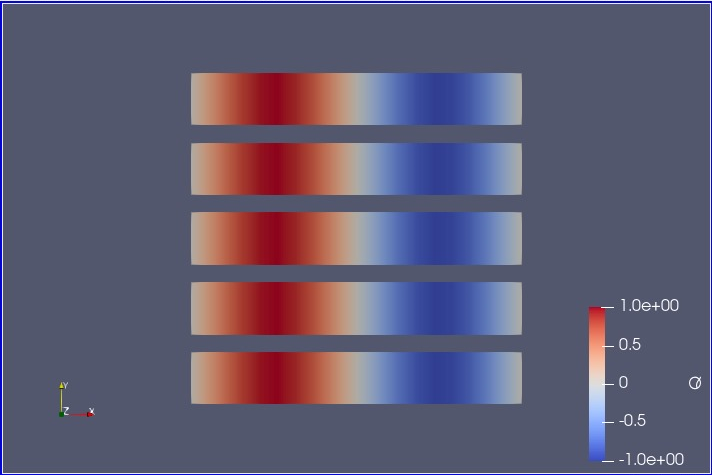
\includegraphics[width=1\linewidth]{Figures/Initial_result.png}
    \caption{Initial values of 15*15 mesh resolution and 5 cores}
    \label{fig:enter-label}
\end{figure}
Every core creates its own output file. With the help of Paraview, these result files can be merged and then shown.  

\subsection{Results of Mesh Resolution}
This section looks into how different mesh resolutions affect computing performance while maintaining a consistent core number. The findings, depicted in Table \ref{tab:veritablo} and Figure \ref{t3}, highlight that the solving time increases at a faster rate than the 'Total node number.' This outcome is consistent with expectations, as increasing the problem size increases communication demands, as evidenced by the observed timing results.

\begin{table}[h]
    \centering
    \begin{tabular}{|c|c|c|c|}
        \hline
        \multirow{2}{*}{\textbf{NX and NY}} & \textbf{Total Node Number: }  & \multirow{2}{*}{\textbf{Time (seconds)}} &  \multirow{2}{*}{\textbf{Infinity norm}} \\
        &\textbf{NX*((NY/CORE NUMBER)+2)*CORE NUMBER} & & \\
        \hline
        50    & 3000 &1.3 & 3.4e-3   \\
        100   & 11000 &3.6 & 9.1e-4 \\
        200   & 42000 &12.8 & 3.2e-4 \\
        400   & 164000 &62.8 & 2.1e-4 \\
        800   & 648000 &428.5 & 9.3e-4 \\
        1200  & 1452000 &1088.4 & 1.3e-3 \\
        1600  & 2576000 &2235.1 & 1.3e-3 \\
        2000  & 4020000 &4123.8 & 1.0e-3 \\
        \hline
    \end{tabular}
    \caption{Mesh resolution vs Computation time when 5 cores used}
    \label{tab:veritablo}
\end{table}
  
\begin{figure}[hbt!]
  \centering
  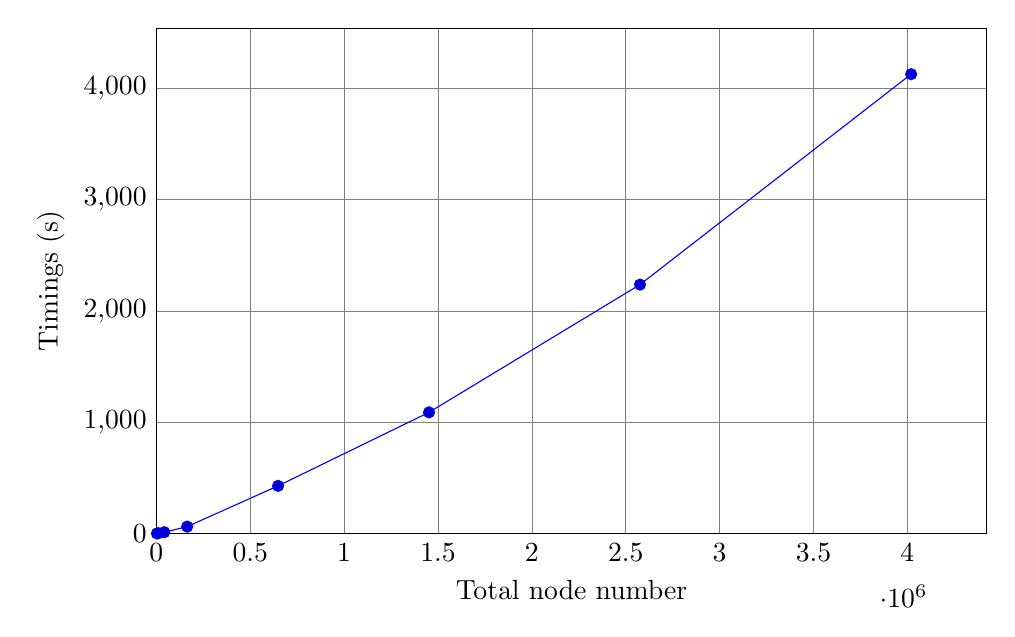
\begin{tikzpicture}
    \begin{axis}[
      width=1\linewidth,
      height=8cm,
      ylabel={Timings (s)},
      xlabel={Total node number},
      grid=major, 
      ymin=0,
      xmin=0,
      grid style={help lines},
    ]

    \addplot coordinates {
        (3000, 1.3)
        (11000, 3.6)
        (42000, 12.8)
        (164000, 62.8)
        (648000, 428.5)
        (1452000, 1088.4)
        (2576000, 2235.1)
        (4020000, 4123.8)
    };

    \end{axis}
  \end{tikzpicture}
  \caption{Total node number vs Computation time when 5 cores used}
  \label{t3}
\end{figure}



\clearpage


\subsection{Results of Comparison the Number of Processes}
Here, we perform a comparison analysis with different numbers of cores but with the same mesh resolutions. The findings, which are shown in Table \ref{tab:veritablo_new} and Figure \ref{t4}, show that as the 'Core number' rises, the decrease in solving time becomes less noticeable. This observation is consistent with expectations, since the increase in core number results in an increased communication overhead that affects the timing outcomes overall. In an ideal parallelization scenario, the curve of computation time versus core number would ideally be a straight line. However, deviations from linearity indicate that higher core numbers are associated with higher communication costs. Analyzing these patterns in more detail might provide ways to improve the parallelization approach. 
\begin{table}[h]
    \centering
    \begin{tabular}{|c|c|c|c|}
        \hline
        \multirow{2}{*}{\textbf{Core number}} & \textbf{Total Node Number: }  & \multirow{2}{*}{\textbf{Time (seconds)}} &  \multirow{2}{*}{\textbf{Infinity norm}} \\
        &\textbf{NX*((NY/CORE NUMBER)+2)*CORE NUMBER} & & \\
        \hline
2	&	362400	&	332.7	&	1.90E-04	\\
3	&	363600	&	225.6	&	2.00E-04	\\
4	&	364800	&	215.5	&	3.80E-04	\\
5	&	366000	&	161.8	&	6.00E-04	\\
6	&	367200	&	151.1	&	1.20E-03	\\

        \hline
    \end{tabular}
    \caption{Core number vs Computation time when NX = 600 }
    \label{tab:veritablo_new}
\end{table}

\begin{figure}[hbt!]
  \centering
  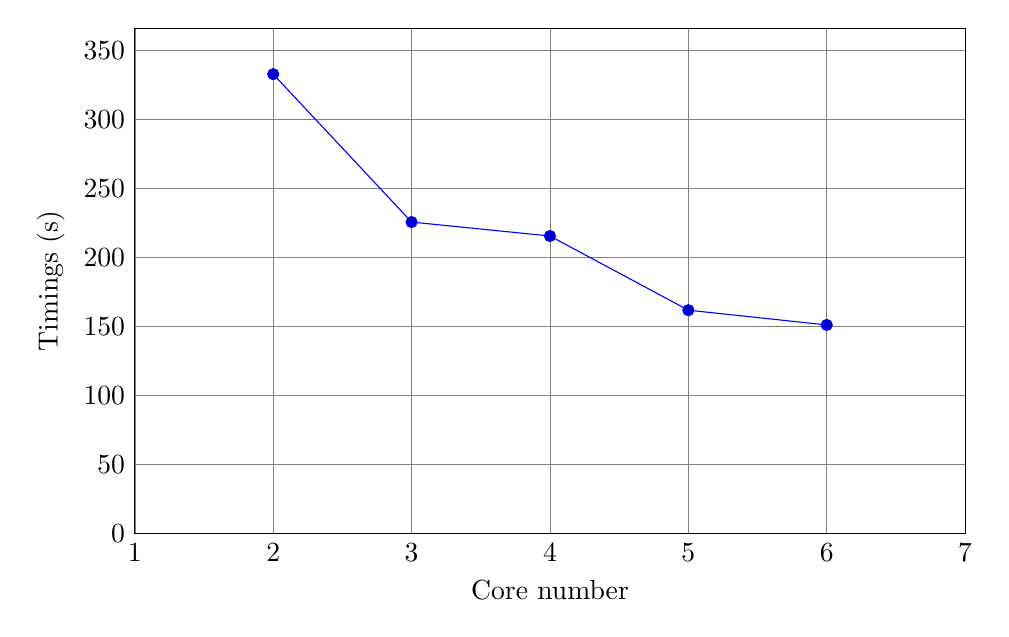
\begin{tikzpicture}
    \begin{axis}[
      width=1\linewidth,
      height=8cm,
      ylabel={Timings (s)},
      xlabel={Core number},
      grid=major, 
      ymin=0,
      xmin=1,
      xmax=7,
      grid style={help lines},
    ]

    \addplot coordinates {
(	2	,	332.7	)
(	3	,	225.6	)
(	4	,	215.5	)
(	5	,	161.8	)
(	6	,	151.1	)

    };

    \end{axis}
  \end{tikzpicture}
  \caption{Core number vs Computation time when NX = 600}
  \label{t4}
\end{figure}



\clearpage

\subsection{Strong Scaling Analysis}

The performance improvement is expressed in terms of \(T_1 / T_P\) in the strong scaling analysis shown in Figure \ref{t5}, where \(T_1\) represents the execution time on a single core and \(T_P\) represents the execution time with \(P\) cores. The 'Strong Scaling' curve represents the actual strong scaling behavior observed during the simulation, while the 'Ideal' curve illustrates the theoretically perfect scaling if there were no overhead or communication costs.

The outcomes show some degree of scalability in the parallelization of the 2D wave equation solver using the MPI toolkit. However, deviations from the ideal curve suggest the presence of overhead or communication costs associated with parallel execution. Further investigations into these areas might shed light on possible improvements for increased scalability.


\begin{figure}[hbt!]
  \centering
  \begin{tikzpicture}
    \begin{axis}[
      width=1\linewidth,
      height=8cm,
      ylabel={T_1 / T_P},
      xlabel={Core number},
      grid=major, 
      ymin=1,
      xmin=1,
      xmax=7,
      grid style={help lines},
    ]

    \addplot coordinates {
(	2	,	2	)
(	3	,	2.949468085	)
(	4	,	3.087703016	)
(	5	,	4.112484549	)
(	6	,	4.403706155	)


    };
    \addlegendentry{Strong Scaling};
    
    \addplot coordinates {
(	2	,	2		)
(	3	,	3		)
(	4	,	4		)
(	5	,	5		)
(	6	,	6		)
    };
    \addlegendentry{Ideal};
    
    \end{axis}
  \end{tikzpicture}
  \caption{Strong Scaling Result with respect to 2 core solution time when NX = 600}
  \label{t5}
\end{figure}

\clearpage

\section{Comments and Conclusion}

In this work, we carried out a thorough investigation of the C-based parallelized 2D wave equation solver using the MPI library. The study concentrated on evaluating the effect of total node numbers on computing time, comparing performance across various mesh resolutions, and strong scaling with varying core counts.

The strong scaling analysis revealed that, as expected, the parallelization efficiency diminishes as the core number increases. This phenomenon is explained by the increased communication overhead that comes with more cores. Disturbances from the optimal scaling curve indicate prospects for optimizing the parallelization approach and reducing communication expenses.

Additionally, the examination of mesh resolution indicated that the solving time increases at a faster rate than the total node number. This discovery is consistent with the expected result, since higher problem sizes result in increased communication requirements. Understanding these trends is crucial for optimizing the algorithm's performance under varying computational conditions.

In conclusion, our results provide valuable insights into the behavior of the parallelized 2D wave equation solver. 


\printbibliography

\end{document}
